% Options for packages loaded elsewhere
\PassOptionsToPackage{unicode}{hyperref}
\PassOptionsToPackage{hyphens}{url}
%
\documentclass[
  9pt,
  ignorenonframetext,
]{beamer}
\usepackage{pgfpages}
\setbeamertemplate{caption}[numbered]
\setbeamertemplate{caption label separator}{: }
\setbeamercolor{caption name}{fg=normal text.fg}
\beamertemplatenavigationsymbolsempty
% Prevent slide breaks in the middle of a paragraph
\widowpenalties 1 10000
\raggedbottom
\setbeamertemplate{part page}{
  \centering
  \begin{beamercolorbox}[sep=16pt,center]{part title}
    \usebeamerfont{part title}\insertpart\par
  \end{beamercolorbox}
}
\setbeamertemplate{section page}{
  \centering
  \begin{beamercolorbox}[sep=12pt,center]{part title}
    \usebeamerfont{section title}\insertsection\par
  \end{beamercolorbox}
}
\setbeamertemplate{subsection page}{
  \centering
  \begin{beamercolorbox}[sep=8pt,center]{part title}
    \usebeamerfont{subsection title}\insertsubsection\par
  \end{beamercolorbox}
}
\AtBeginPart{
  \frame{\partpage}
}
\AtBeginSection{
  \ifbibliography
  \else
    \frame{\sectionpage}
  \fi
}
\AtBeginSubsection{
  \frame{\subsectionpage}
}
\usepackage{lmodern}
\usepackage{amsmath}
\usepackage{ifxetex,ifluatex}
\ifnum 0\ifxetex 1\fi\ifluatex 1\fi=0 % if pdftex
  \usepackage[T1]{fontenc}
  \usepackage[utf8]{inputenc}
  \usepackage{textcomp} % provide euro and other symbols
  \usepackage{amssymb}
\else % if luatex or xetex
  \usepackage{unicode-math}
  \defaultfontfeatures{Scale=MatchLowercase}
  \defaultfontfeatures[\rmfamily]{Ligatures=TeX,Scale=1}
\fi
\usetheme[]{Goettingen}
\usecolortheme{rose}
% Use upquote if available, for straight quotes in verbatim environments
\IfFileExists{upquote.sty}{\usepackage{upquote}}{}
\IfFileExists{microtype.sty}{% use microtype if available
  \usepackage[]{microtype}
  \UseMicrotypeSet[protrusion]{basicmath} % disable protrusion for tt fonts
}{}
\makeatletter
\@ifundefined{KOMAClassName}{% if non-KOMA class
  \IfFileExists{parskip.sty}{%
    \usepackage{parskip}
  }{% else
    \setlength{\parindent}{0pt}
    \setlength{\parskip}{6pt plus 2pt minus 1pt}}
}{% if KOMA class
  \KOMAoptions{parskip=half}}
\makeatother
\usepackage{xcolor}
\IfFileExists{xurl.sty}{\usepackage{xurl}}{} % add URL line breaks if available
\IfFileExists{bookmark.sty}{\usepackage{bookmark}}{\usepackage{hyperref}}
\hypersetup{
  pdftitle={BIOS6643 Longitudinal},
  pdfauthor={EJC},
  hidelinks,
  pdfcreator={LaTeX via pandoc}}
\urlstyle{same} % disable monospaced font for URLs
\newif\ifbibliography
\setlength{\emergencystretch}{3em} % prevent overfull lines
\providecommand{\tightlist}{%
  \setlength{\itemsep}{0pt}\setlength{\parskip}{0pt}}
\setcounter{secnumdepth}{-\maxdimen} % remove section numbering
\AtBeginSubsection{}
\AtBeginSection{}
\ifluatex
  \usepackage{selnolig}  % disable illegal ligatures
\fi

\title{BIOS6643 Longitudinal}
\subtitle{L13 Modeling independent or correlated}
\author{EJC}
\date{}
\institute{Department of Biostatistics \& Informatics}

\begin{document}
\frame{\titlepage}

\begin{frame}[allowframebreaks]
  \tableofcontents[hideallsubsections]
\end{frame}
\hypertarget{introduction-modeling-independent-or-correlated}{%
\section{1. Introduction: Modeling independent or
correlated}\label{introduction-modeling-independent-or-correlated}}

\begin{frame}{1.0 Introduction}
\protect\hypertarget{introduction}{}
This set of notes discusses models that can be used for \textbf{outcome
variables that are not normally distributed}. Methods for modeling
non-normal correlated data are also discussed in BIOS7712. We have
learned how to use linear mixed models to fit clustered data with
continuous and approximately normally distributed outcome variables. The
models are versatile in handling random effects as well as repeated
measures over time. For other types of outcome variables that involve
clustered data, such as counts or binary outcomes, we can use
generalized estimating equations (GEE) or employ generalized linear
mixed models (GzLMM) as discussed in this chapter.

Sometimes we can still employ normal theory models even when the outcome
variable is non-continuous or non-normal. For example, a count outcome
with a wide range of observed values not too close to zero \textbf{may
be well approximated by the normal curve}. In other cases we might be
able to apply a \textbf{transformation} to a non-normal outcome so that
it is approximately normal. In particular, outcome variables with
right-skewed distributions are very common (e.g., cell counts),
especially when there is a lower bound (typically zero). A natural
\textbf{log transformation} might make the distribution approximately
normal. But \textbf{how then are effects from the model interpreted?}
This will be examined in more detail in the section on interpreting
effects from loglinear and logistic models.
\end{frame}

\hypertarget{determining-when-and-when-not-to-use-normal-theory-methods}{%
\section{2. Determining when and when not to use normal theory
methods}\label{determining-when-and-when-not-to-use-normal-theory-methods}}

\begin{frame}{2.0 Determining when and when not to use normal theory
methods}
\protect\hypertarget{determining-when-and-when-not-to-use-normal-theory-methods-1}{}
For a given outcome variable, a normal-theory model (e.g., GLM, LMM) may
work adequately even if the observed data are not perfectly normal.
Typically, the model fit will be fairly robust to violations of the
normal assumption as long as the distribution is not too skewed or does
not have a high percentage of data on one or more individual values, or
when sample sizes are large enough that the central limit theorem comes
into play.
\end{frame}

\begin{frame}{2.1 Consider the following examples of response variables
and how you might model them}
\protect\hypertarget{consider-the-following-examples-of-response-variables-and-how-you-might-model-them}{}
\begin{enumerate}
\item
  \(Y\) = FEV1: slightly right skewed; true lower bound of 0 although
  \(P(Y=0)=0\) or negligible for a non-error blow.
\item
  \(Y\) = forced exhaled nitric oxide (FeNO): moderately right-skewed;
  lower bound of 0 but \(P(Y=0)=0\) or negligible.
\item
  \(Y\) = expenditures for health clinics; can be considered continuous;
  right skewed but with \(P(Y=0)>0\) and possible that \(P(Y=0)\gg 0\)
  (e.g., 20\% or more).
\item
  \(Y\) = whether child had an asthma exacerbation in a given week
  (y/n).
\item
  \(Y\) = percentage of patients that adhere to doctor's directions,
  based on large n.
\item
  \(Y\) = number of times albuterol was used in a day by a child to
  treat asthma. Counts of use typically range from 0 to 6, but most
  commonly are 0, 1 or 2.
\end{enumerate}
\end{frame}

\hypertarget{generalized-linear-models-gzlm-an-introduction}{%
\section{3. Generalized linear models (GzLM), an
introduction}\label{generalized-linear-models-gzlm-an-introduction}}

\begin{frame}{3.0 Generalized linear models (GzLM), an introduction}
\protect\hypertarget{generalized-linear-models-gzlm-an-introduction-1}{}
When a normal-theory model is clearly not suitable for the outcome even
after transforming, one possibility, \textbf{if the outcome variable can
be modeled by a distribution from the exponential family (EF)}, is to
use \textbf{general-ized linear models (GzLM)}. Generalized Linear
Models is \textbf{one of the most important classes of statistical
models} and \textbf{one of several huge innovations in statistics in the
1970's and 80's}, well represented by the landmark paper by
\textbf{Nelder and Wedderburn in 1972}. {[}Survival analysis (Cox, 1972)
and linear mixed models (Laird and Ware, 1982) also made big leaps in
their development during this time.{]} GzLMs generalize linear models
for use with non-normal outcomes. As with most regression methods, in
GzLMs we consider both the mean and variance of \(Y\) conditional on
\(\pmb X\), although this is usually not explicitly written.
\end{frame}

\begin{frame}{3.1 \textbf{Notation}}
\protect\hypertarget{notation}{}
Since notation is very complicated with GzLMs, a summary is given below
to highlight some of the key elements.

\(Y_i\): Random variable outcomes, \(i=1,\ ...\ ,\ n\)\\
\(y_i\): Observed outcomes\\
\(\pmb x_i^r\): Covariate vector for subject \(i\), the \(i\)th row of
\(\pmb X\)\\
\(x_{ij}\): Covariate value for subject \(i\) and covariable \(j\)\\
\(\pmb \beta\): Regression parameter vector for GzLM\\
\alert {$\mu_i =E[Y_i]$: mean outcome for subject $i$}\\
\(\eta_i =\pmb x_i^r \pmb \beta\): linear predictor for subject \(i\)
for GzLM\\
\(g\): Link function for GzLM, \(\eta_i=g(\mu_i)\) or equivalently
\(\mu_i=g^{-1}(\eta_i)\).\\
\(\theta\): Canonical parameter in EF, defines canonical link
\(\theta(\mu)\) for \(\mathcal {EF}\)\\
\(\phi\): Scale parameter; either a fixed parameter in the density, or a
parameter artificially added in Quasilikelihood\\
\(f_Y (y;\ \theta,\ \phi)\): Density in \(\mathcal {EF}\) form\\
\(\mathcal L(\pmb \theta,\ \phi;\ \pmb y)\): Likelihood\\
\(\mathcal D(\pmb \theta,\ \phi;\ \pmb y)\): Deviance

Here, the acronym GzLM is used for generalized linear models, while GLM
is used for general linear models. But note that some authors refer to
generalized linear models as `GLM' and general linear models are often
just referred to as `linear models', or `LM'. In R software, the
\emph{glm()} function will fit a generalized linear model, while lm fits
a general linear model.
\end{frame}

\begin{frame}{3.2 Motivation and examples}
\protect\hypertarget{motivation-and-examples}{}
There are many types of outcomes that one may be interested in modeling
that are not normally distributed, or even continuous. For example:
\textbf{number of visits to ER each day}; number of asthma inhaler uses
each day; disease exacerbation: yes/no.

What about using the following GLM to model such data?\\
\(Y_i=\pmb x_i^r \pmb \beta+\epsilon_i=\sum_{j=1}^p x_{ij} \beta_j +\epsilon_i\)

But note that such a model \textbf{will not generate integer
(e.g.~count) data, nor binary (0/1) data}.

\textbf{Historical (early) `solutions'} to dealing with inadequacies of
GLMs in modeling non-normal data included use of variance stabilizing
transformations and empirical transformations of the response variable.
But these clearly have their limitations.
\end{frame}

\begin{frame}{3.3 Link functions}
\protect\hypertarget{link-functions}{}
The modern solution to the modeling issues discussed above is GzLMs,
proposed by \textbf{Nelder \& Wedderburn (1972)}. The key idea is
\textbf{to consider the distribution of the response variable rather
than including an additive error term}. For example, for the normal, we
can \textbf{rewrite}

\(Y_i=\pmb x_i^r \pmb \beta+\epsilon_i,\  \epsilon_i\sim \mathcal N(0,\ \sigma^2)\)
\textbf{as} \(Y_i\sim \mathcal N(\pmb x_i^r \pmb \beta,\ \sigma^2)\).

For the \(\mathcal {Poisson}\), there is one parameter so we could
consider \(Y_i \sim \mathcal {Pois} (\pmb x_i^r \pmb \beta)\).

Now we have a model where \textbf{response values are integer valued}.
But one obvious problem with this is that
\textbf{\(\pmb x_i^r \pmb \beta\) isn't necessary positive}. One way to
avoid this problem is to consider
\(Y_i \sim \mathcal {Pois} \big(e^{\pmb x_i^r \pmb \beta} \big)\) or
equivalently,

\[Y_i \sim \mathcal {Pois} (\mu_i)\ with\ \ ln(\mu_i)=\pmb x_i^r \pmb \beta \ \ \ \ \ \ \ [1]\]

Thus, instead of setting \(E[Y_i]=\mu_i=\pmb x_i^r \pmb \beta\), we find
a function of \(\pmb x_i^r \pmb \beta\) so that the parameter space of
the response mean is maintained in the model.
\end{frame}

\begin{frame}{}
\protect\hypertarget{section}{}
\textbf{Let \(g\) denote the link function between the linear predictor,
\(\pmb x_i^r \pmb \beta\), and the mean, \(\mu_i\)}, so that

\[g(\mu_i)=\pmb x_i^r \pmb \beta. \ \ \ \ \ \ \ [2]\]

For the \(\mathcal {Poisson}\), the link function expressed in {[}1{]}
is \(g(\mu) = ln(\mu)\). This link is intuitive because it keeps the
\(\mathcal {Poisson}\) mean positive in the model. It can also be shown
that the canonical link or natural link (discussed more ahead) for the
\(\mathcal {Poisson}\) distribution is in fact the natural log link.
Count outcomes can often be modeled using a \(\mathcal {Poisson}\)
distribution, although it is often necessary to add a dispersion
parameter into the model (also discussed later). Regression of a
\(\mathcal {Poisson}\) variable on one or more predictors is often
referred to as \(Poisson regression\). Another form of {[}2{]} is
\(\mu_i=g^{-1} (\pmb x_i^r \pmb \beta)\). For the
\(\mathcal {Poisson}\), we have
\(\mu_i=g^{-1} (\pmb x_i^r \pmb \beta)=e^{\pmb x_i^r \pmb \beta}\).

A \textbf{plot} of this function with one covariate and \(\beta_0=0\)
and \(\beta_1=1\) is presented in \emph{Figure 1}, left panel.
\end{frame}

\begin{frame}{}
\protect\hypertarget{section-1}{}
For the \textbf{binomial}, consider
\(\hat p_i= \frac {Y_i} {n_i},\ where\ Y_i \sim \mathcal {Bin} (n_i,\ p_i )\).
Of course \(p\) must be bound between 0 and 1 and intuitively would be a
continuous function of \(\pmb x_i^r\). In order to maintain these
characteristics, one possibility is to set

\[p_i=\frac {e^{\pmb x_i^r \pmb \beta}} {1+e^{\pmb x_i^r \pmb \beta} }. \ \ \ \ \ \ [3]\]

Function {[}3{]} is plotted for one continuous covariate in the right
panel of \emph{Figure 1}, with \(\beta0 = 0\) and \(\beta1=1\); this
demonstrates the signature `slanted S' shape. However, for certain
applications, this may not be apparent since the range of \(x\) values
may only cover a portion of the `S'.
\end{frame}

\begin{frame}{Figure 1: plot of mean functions for log (left panel) and
logit (right panel) links.}
\protect\hypertarget{figure-1-plot-of-mean-functions-for-log-left-panel-and-logit-right-panel-links.}{}
\begin{center}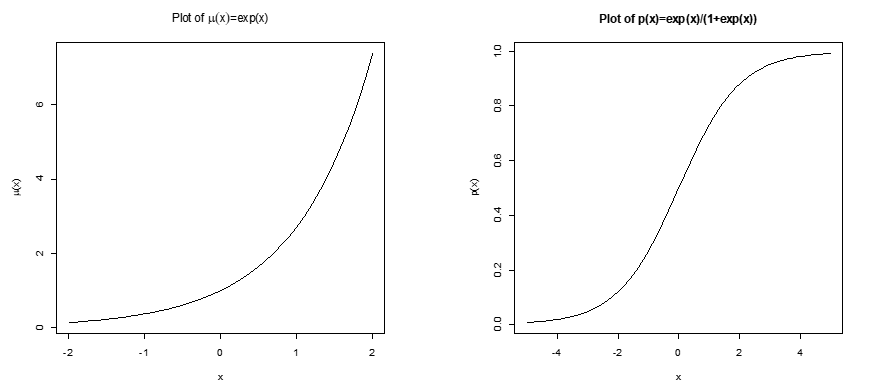
\includegraphics[width=0.4\linewidth]{figs_L13/poisson} \end{center}

Note that for the\(\mathcal {Binomial}\) proportion \(\hat p_i\),
\(E[\hat p_i] = \frac {n_i p_i } {n_i} = p_i\), so {[}3{]} expresses
\(g^{-1}\). Rearranging {[}3{]} in terms of the linear predictor yields
\(g(\mu_i )=ln \big[\frac {\mu_i} {1–\mu_i} \big]=logit(\mu_i)\), which
is the canonical link function for a\(\mathcal {Binomial}\) proportion.
When \(n_i=1\) for all \(i\), we have binary responses
\([Y_i \sim \mathcal {Bernoulli}(p_i),\ i = 1,\ ...,\ n]\). Modeling of
a binary outcome as a function of one or more predictors (at least one
usually continuous) is called \textbf{logistic regression}. In our
model, we estimate \(\pmb \beta\), which will then provide estimates of
the probability that \(Y\) will be 0 or 1, through {[}3{]}.
\end{frame}

\begin{frame}{}
\protect\hypertarget{section-2}{}
Note that for normal outcomes, the GzLM with normal distribution and
identity link is
\(Y_i\sim \mathcal N(\pmb x_i^r \pmb \beta,\ \sigma^2)\), which is
equivalent to the usual GLM.

To summarize, in a GLM, the mean part of the model is \(\pmb X\beta\),
or \(\mu\). But as illustrated above, for outcomes that are not normally
distributed, it is not always best to set these quantities equal. To
distinguish the terms we'll call \(\pmb X\beta\) the linear predictor,
sometimes denoted as \(\eta\). For subject \(i\), the linear predictor
is the scalar \(\eta_i=\pmb x_i^r \pmb \beta\), where \(x_i^r\) is the
\(i\)th row of \(\pmb X\).
\end{frame}

\begin{frame}{3.4 \textbf{Components of the GzLM}}
\protect\hypertarget{components-of-the-gzlm}{}
\textbf{In general, a GzLM looks like
\(Y_i \sim \mathcal {EF}(g^{-1} (\pmb x_i^r \pmb \beta),\ \phi)\)} where
\(\phi\) is a vector of other parameters, e.g.~\(\sigma^2\) for normal
distributions, and \textbf{`EF' refers to a distribution from the class
of exponential family distributions, parameterized so that the first
argument is the mean}. There are \textbf{three main components} to a
GzLM:

\begin{enumerate}
\item
  \textbf{Random component}: \(Y_i\sim \mathcal {EF}\)\\
  \textbf{\(\mathcal {EF}\)} = ``Exponential family distribution''\\
  E.g., \(\mathcal {Poisson ,\ Binomial,\ Normal,\ Gamma}\)
\item
  \textbf{Systematic component}: \(\pmb x_i^r \pmb \beta\)\\
  Sometimes called \textbf{`Linear Predictor'}, sometimes denoted as
  \(\eta_i=\pmb x_i^r \pmb \beta\)\\
  E.g., includes covariates, groups, treatments, interactions, etc.
\item
  \textbf{Link function}: \(g\)\\
  Links systematic and random components, ie covariates and mean\\
  \(E(Y_i)=\mu_i=g^{-1} (\eta_i)=g^{-1} (\pmb x_i^r \pmb \beta)\), or
  equivalently \(g(\mu_i)=\eta_i\).\\
  Also keeps mean of random distribution in right space.\\
  E.g. \(log\) for \(\mathcal {Poisson}\), \(logit\) for
  \(\mathcal {Binomial}\)
\end{enumerate}
\end{frame}

\begin{frame}{3.5 Exponential family distributions}
\protect\hypertarget{exponential-family-distributions}{}
An \textbf{exponential family distribution} has density of the form

\[
f_Y (y;\ \theta,\ \phi)=exp\Big(\frac {y\theta-b(\theta)} {a(\phi)} +c(y,\phi)\Big)
\]

Note that \(b(\theta)\) occurs alone, with no \(y\)'s, and
\(c(y,\ \phi)\) occurs alone, with no \(\theta\)'s; \(\theta\) may be a
vector parameter, though in common cases it is a scalar. Here we
consider it as a scalar and leave it unbolded.

The link function \(g\) for which \(g(\mu)=\theta\) is called the
canonical link. This is typically the link function used to relate the
mean of \(Y\) to the covariates in the GzLM. In other words, when the
canonical link is used in the GzLM,
\(\theta_i=\eta_i=\pmb x_i^r \pmb \beta\) (considering subject \(i\)).
\end{frame}

\begin{frame}{}
\protect\hypertarget{section-3}{}
There may be other \textbf{nuisance parameters}. One particular case is
a \textbf{scale parameter \(\phi\)}. In some common situations
(e.g.~\(\mathcal {Poisson}\)), \(a(\phi)=1\). The scale parameter
\(\phi\) is considered fixed throughout most of the analyses. A scale
parameter can also be added in cases where \(a(\phi)=1\)
(e.g.~\(\mathcal {Poisson}\)). This does not give a true probability
distribution, but it can be useful in practice and is called
\textbf{Quasilikelihood estimation}, which will be discussed ahead.

Some \textbf{general results} are available for exponential families.
For example, \(E[Y_i]=\mu=b' (\theta)\) and
\(Var[Y_i]=b''(\theta)a(\phi)\).

For practice: determine the exponential form and related quantities for
the Normal case. (The \(\mathcal {Poisson}\) and\(\mathcal {Binomial}\)
cases will be given as homework.)
\end{frame}

\hypertarget{estimation}{%
\section{3.6 Estimation}\label{estimation}}

\begin{frame}{3.6.1 Likelihood and score equations}
\protect\hypertarget{likelihood-and-score-equations}{}
The \textbf{likelihood} for data \(y_1,\ ...,\ y_n\) based on iid
responses from a member of the exponential family is

\[
\mathcal L(\theta,\ \phi;\ y) = \prod_{i=1}^n f_Y (y_i;\ \theta_i,\ \phi) =\prod_{i=1}^n exp  \Big( \frac {y_i \theta_i-b(\theta_i)} {a(\phi)}+c(y_i,\ \phi)\Big) 
\]

For \textbf{maximum likelihood estimation}, we take the derivative of
logL with respect to \(\pmb \beta\) (embedded in theta in the equations
above), set it to 0, and \textbf{solve for \(\pmb \beta\), the MLE}.

First, let's consider the contribution to the likelihood from subject
\(i\):

\[
\mathcal l_i= ln(\mathcal L_i)= ln[f(y_i;\ \theta_i,\ \phi)] = \frac {y_i \theta_i-b(\theta_i )} {a(\phi)} + c(y_i,\ \phi)
\]

Using the chain rule,

\[
\frac {\partial \mathcal l_i} {\partial\beta_j} = \frac {\partial \mathcal l_i} {\partial\theta_i } \frac {\partial\theta_i} {\partial\mu_i } \frac {\partial\mu_i} {\partial\eta_i } \frac {\partial\eta_i} {\partial\beta_j }
\]
\end{frame}

\begin{frame}{}
\protect\hypertarget{section-4}{}
Using this, we can arrive at

\[
\frac {\partial \mathcal l_i} {\partial\beta_j }=\frac {(y_i-\mu_i)x_{ij}} {Var[Y_i]} \frac {\partial\mu_i} {\partial\eta_i}
\]

Hence, the score equations are

\[
\frac {\partial \mathcal L} {\partial\beta_j} = \sum_{i=1}^n \frac {(y_i-\mu_i)x_{ij}} { Var[Y_i]} \frac {\partial\mu_i} {\partial\eta_i} =0 ,\     j=1,\ ...,\ p .
\]

Note that the \(\mathcal {Beta}\) parameters are contained in \(\mu_i\).
\(Var[Y_i]\) above can be expressed as a function of the mean which has
a specific form for a given distribution for \(Y\) (e.g.,
\(Var[Y_i]=\mu\) for the \(\mathcal {Poisson}\)). \textbf{Solving these
equations for \(\pmb \beta\) with data at hand can be accomplished using
iterative algorithms}, which are described below.
\end{frame}

\begin{frame}{3.6.2 Newton Raphson and Fisher Scoring algorithms}
\protect\hypertarget{newton-raphson-and-fisher-scoring-algorithms}{}
For distributions other than the normal, \(\mu_i\) is not a linear
function of \(\pmb \beta\), so there is no closed form solution for
these estimates like there is in the General Linear Model. Thus, finding
numerical maximum likelihood estimates requires using a numerical
optimization search algorithm, such as a Newton-Raphson method or
Fisher's Scoring Algorithm. There is a difference between these
algorithms in that Fisher's Scoring Algorithm uses the \textbf{expected
information matrix} {[}expected value of the \textbf{Hessian matrix},
with elements
\(E \Big[\frac {\partial \mathcal L^2} {\partial\beta_j \partial\beta_k}\Big]\),
while the NR method uses the Hessian matrix itself, called the
\textbf{observed information matrix}. In SAS, you can determine which
approach to use. In fact, it is possible to start the iterations using
the expected information matrix, and then switch over the observed
information matrix by including the SCORING option and specifying at
which iteration the change should be made. When the canonical link is
used, the methods are equivalent (see Nelder and Wedderburn, 1972). For
more detail on the algorithms, see Agresti (2002).
\end{frame}

\begin{frame}{3.6.3 \textbf{Iteratively reweighted least squares}}
\protect\hypertarget{iteratively-reweighted-least-squares}{}
The Fisher Scoring Algorithm applied to the estimating equations above
can be re-expressed as the iteratively reweighted least squares (IRWLS)
algorithm. Below is a rough summary of this algorithm.

A. \textbf{First calculate the LS estimate
\(\pmb {\hat \beta} ^{(0)} = \pmb {\hat \beta}_{LS}\)}. This is
inefficient because variances are unequal and the mean is nonlinear in
parameters, but it provides a good starting value for the algorithm.

B. \textbf{Calculate the variances \(V_i^{(k)}\) of the observations
\(Y_i\)}. Note that in general these \textbf{variances depend on the
means}.

C. \textbf{Construct the n×n diagonal weight matrix} with elements
\(W_{ii}^{(k)}= \frac 1 {V_i^{(k)}} \Bigg(\frac {\partial\mu_i^{(k)}} {\partial\eta_i^{(k)}} \Bigg)^2\).
The derivative term is needed because of the curvature in the link
function (recall that
\(E[Y_i] =\mu_i=g^{-1} (\eta_i)=g^{-1} (\pmb x_i^r \pmb \beta))\).

D. \textbf{Calculate the Weighted Least Squares (WLS) estimate
\(\pmb {\hat \beta}^{(k)} = (\pmb X^{\top} \pmb {WX} )^{-1} \pmb X^{\top} \pmb {Wy}\)}.
The weights account for the unequal variances and the nonlinearity of
\mu\_i with respect to \beta (see C).

E. \textbf{Repeat steps B-D} using the **updated estimate of
\(\pmb \beta^{(k)}\) (\(k\) denotes iteration number). The iteration is
needed because there is no closed form solution.

F.\textbf{Continue to iterate to convergence}. It can be shown that
under quite general conditions, including GzLMs, this algorithm
\textbf{converges to the ML estimate}.
\end{frame}

\begin{frame}{}
\protect\hypertarget{section-5}{}
Note how the \textbf{theory of GzLM's and exponential families was used
to derive this general algorithm}, as opposed to using a general
numerical algorithm (e.g.~Newton Raphson) to find the
\(\pmb {\hat \beta}\) that minimizes the logL function. The latter is
possible but much less efficient, which makes a big difference when
there are many predictors (i.e., elements in \(\pmb \beta\)).
\end{frame}

\begin{frame}{3.6.4 \textbf{MCMC estimation}}
\protect\hypertarget{mcmc-estimation}{}
There is another approach to estimation of GzLMs based on Bayesian
estimation and Markov Chain Monte Carlo (MCMC) simulation methods. This
is implemented in the free software
\href{http://www.mrc-bsu.cam.ac.uk/bugs/}{WinBugs}. There will be one
lecture day devoted to this topic during this course.
\end{frame}

\hypertarget{goodness-of-fit}{%
\section{3.7 Goodness of fit}\label{goodness-of-fit}}

\begin{frame}{3.7.0 Assessing model fit -- goodness of fit statistics
and residuals}
\protect\hypertarget{assessing-model-fit-goodness-of-fit-statistics-and-residuals}{}
There are two general approaches to checking the fit of GzLMs:
Residuals, and goodness of fit statistics. They are related in that the
two main definitions of residuals are each related to the two main
definitions of goodness of fit statistics.
\end{frame}

\begin{frame}{3.7.1 Goodness of fit statistics}
\protect\hypertarget{goodness-of-fit-statistics}{}
\begin{block}{3.7.1.1 Deviance}
\protect\hypertarget{deviance}{}
The deviance is the most important goodness of fit statistic. It
compares the log-likelihood at the MLE with the log-likelihood of the
best possible model, which has one parameter for each data point.

Recall the likelihood for a GzLM is

\[
\mathcal L(\theta,\ \phi;\ y)=\prod_{i=1}^n f_Y (y_i;\ \theta_i,\ \phi) =\prod_{i=1}^n exp \Bigg(\frac {y_i \theta_i-b(\theta_i)} {a(\phi)} + c(y_i,\ \phi)\Bigg) 
\]

where \(\theta_i\) is the natural (or canonical) parameter defined as
\(\theta_i=g(\mu_i)\) with \(E[Y_i]=\mu_i\). The log-likelihood is
\(ln \mathcal L(\theta,\ \phi;\ y)=\sum_{i=1}^n \frac {y_i \theta_i-b(\theta_i)} {a(\phi)}+c(y_i,\phi)\)
and the \((-2)\) difference between evaluating this at the best possible
model (`full model') where for each \(i\), \(\mu_i=y_i\) and
\(\theta_i=\tilde \theta_i\), and at the MLE \(\pmb \theta\), is defined
as the Deviance:

\[
\mathcal D(\pmb \theta,\ \phi;\ \pmb y)=-2[ln \mathcal L(\pmb {\hat \theta},\ \phi;\ \pmb y) - ln \mathcal L(\pmb {\tilde \theta},\ \phi;\ \pmb y)] = -2\sum_{i=1}^n \frac {[y_i ({ \hat \theta} _i- \tilde \theta_i)-(b(\hat \theta_i)-b(\tilde \theta _i))]} {a(\phi)}.
\]
\end{block}
\end{frame}

\begin{frame}{}
\protect\hypertarget{section-6}{}
\begin{block}{3.7.1.1 Deviance}
\protect\hypertarget{deviance-1}{}
\[
\mathcal D(\pmb \theta,\ \phi;\ \pmb y)=-2[ln \mathcal L(\pmb {\hat \theta},\ \phi;\ \pmb y) - ln \mathcal L(\pmb {\tilde \theta},\ \phi;\ \pmb y)] = -2\sum_{i=1}^n \frac {[y_i ({ \hat \theta} _i- \tilde \theta_i)-(b(\hat \theta_i)-b(\tilde \theta _i))]} {a(\phi)}.
\]

This looks like a likelihood ratio statistic since the difference in
log-likelihoods is like the log of the likelihood ratio, and in fact is
really just another name for a particular \((-2ln)\) likelihood ratio.
So the usual Chi-square asymptotic results hold:

\(\mathcal D(\pmb \theta,\ \phi;\ \pmb y) \sim \chi_{(n-p)}^2\)

Usually the deviance is used for comparing models, similar to F-tests or
likelihood ratio tests in GLMs, see next section.
\end{block}
\end{frame}

\begin{frame}{}
\protect\hypertarget{section-7}{}
\begin{block}{3.7.1.2 Pearson Chi-square}
\protect\hypertarget{pearson-chi-square}{}
The Pearson Chi-square statistic is defined, and has asymptotic
distribution

\[
\chi^2 \equiv \sum_{i=1}^n \frac {(y_i- \hat \mu_i )^2} {Var[\hat \mu_i]} \sim \chi_{(n-p)}^2
\]

where \(Var[\hat \mu_i]=Var[Y_i]\) is a function of \(\mu_i\), evaluated
at \(\hat \mu_i\). (Remember that the variance may depend on the mean.)

Several books caution that the asymptotic properties of deviance and
Pearson Chi-square statistics may not be good even for moderate sample
sizes.
\end{block}
\end{frame}

\begin{frame}{3.7.2 Residuals}
\protect\hypertarget{residuals}{}
Residuals for non-normal GzLMs are more challenging than for normal GLMs
because the concept of residuals is harder to define and the properties
of various proposed residuals are not always great.

Residuals in normal GLMs can be thought of as estimates of the additive
errors:

\begin{itemize}
\item
  Model:
  \(Y_i=\pmb x_i^r \pmb \beta+\epsilon_i=\sum_{j=1}^p x_{ij} \beta_j +\epsilon_i\)
\item
  Residuals: \(r_i=y_i-\pmb x_i^r \pmb {\hat \beta}\)
\end{itemize}

What is the corresponding quantity for models defined with
\(\mathcal {EF}\) distributions, as below?

\begin{itemize}
\tightlist
\item
  \(Y_i\sim \mathcal {EF}(g^{-1} (\pmb x_i^r \pmb \beta),\ \phi)\)
\end{itemize}
\end{frame}

\begin{frame}{}
\protect\hypertarget{section-8}{}
Each of the two main goodness of fit statistics, Pearson (or
chi-squared) and Deviance, is a sum over all observations. The
contributions to the sum are defined as the residuals of each type.

\begin{itemize}
\item
  Pearson (or Chi-square) residuals:
  \(r^P _i\equiv \sqrt\frac {y_i-\mu_i} {V[\mu_i]}\)
\item
  Deviance residuals:
  \(r^D _i\equiv \sqrt {d_i}\big(sign(y_i-\mu_i)\big)\)
\end{itemize}

where \(d_i\) is the \(i\)-th contribution to the deviance.There are
standardized versions of each of these, so that each residual has
(asymptotic) variance 1. Residuals are analyzed as in usual GLMs,
graphically. They can be obtained in GENMOD using the OUTPUT statement.
\end{frame}

\hypertarget{inference}{%
\section{\texorpdfstring{3.8
\textbf{Inference}}{3.8 Inference}}\label{inference}}

\begin{frame}{3.8.0 \textbf{Inference}}
\protect\hypertarget{inference-1}{}
The two general tools for constructing significance tests and confidence
intervals, likelihood ratios and Wald methods, continue to be useful for
GzLMs. In addition, the usual AIC and BIC criteria are available for
comparing non-nested models. All of these results rely on some degree of
asymptotic argument. All of these can be computed in SAS using PROC
GENMOD or in R using glm.
\end{frame}

\begin{frame}{3.8.1 Likelihood ratios}
\protect\hypertarget{likelihood-ratios}{}
Likelihood ratio tests are useful for nested models, and are constructed
and interpreted as usual, with the \(-2 log \mathcal L\) difference
being asymptotically distributed as a \(\chi^2\) with degrees of freedom
equal to the difference in number of parameters in the two models. Note
that this is equivalent to the difference in deviances between the
models since the saturated model term in the deviance cancels out in the
subtraction.

Confidence intervals for individual parameters can be based on
likelihood ratios, using profile likelihood methods.
\end{frame}

\begin{frame}{3.8.2 Wald statistic}
\protect\hypertarget{wald-statistic}{}
Wald tests and CIs are based on the form

\(Z=\frac {\hat \beta_j-\beta_j}{\widehat SE(\hat \beta_j)}\) for tests
and \(\beta_j-\beta_j \pm z_{(1-\alpha/2)} \widehat SE(\beta_j)\) for
CIs.

These rely on the ability of the theory to correctly estimate the
standard errors, and on the asymptotic normality of the sampling
distributions of the estimators.

The standard errors for ML estimates are obtained from
\(Cov[\pmb {\hat \beta}]\) which in ML theory is obtained from the
\emph{negative inverse of the information matrix}. In GzLMs this is
obtained from \((\pmb {X^{\top}WX})^{-1}\) in the final step of the
IRWLS algorithm (there is sometimes a scale parameter involved too).
\end{frame}

\begin{frame}{3.8.3 AIC and BIC}
\protect\hypertarget{aic-and-bic}{}
The general penalized likelihood model comparison statistics
\(AIC=-2 ln \mathcal L(\pmb \theta,\ \phi;\ \pmb y)+2p\),
\(BIC=-2 ln \mathcal L(\pmb \theta,\ \phi;\ \pmb y)+ln(n)p\) are useful
for comparing non-nested GzLMs. BIC selects models with fewer parameters
than AIC. A difference of about 2 in AIC is often considered an
improvement between two models. I don't know what the corresponding
value is for BIC.

There are two cases where caution is needed:

\begin{itemize}
\item
  I don't know if these have been extended to models including scale
  parameters estimated by quasilikelihood (see below).
\item
  For longitudinal data it is not clear what value of n should be used
  in BIC. It should be something between the number of observations and
  the number of subjects (see Jones RH, 2011, Bayesian information
  criterion for longitudinal and clustered data, Statistics in Medicine
  online.)
\end{itemize}
\end{frame}

\hypertarget{over--and-under-dispersion-and-quasilikelihood}{%
\section{3.9 Over- and under-dispersion and
quasilikelihood}\label{over--and-under-dispersion-and-quasilikelihood}}

\begin{frame}{3.9.1 Introduction}
\protect\hypertarget{introduction-1}{}
The \(\mathcal {Poisson}\) distribution is the standard first choice for
count data in the sample space \((0,\ 1,\ 2,\ ...)\), and
the\(\mathcal {Binomial}\) for counts in \((0,\ 1,\ ...,\ n)\). These
situations differ from the Normal, where there is a separate parameter
\(\sigma^2\) that controls the variance independently of the mean.

Recall the theoretical relationships

\begin{itemize}
\item
  Poisson: \(Var[Y]=\mu\)
\item
  Binomial: \(Var[Y]= n\mu(1-\mu)\).
\end{itemize}

These are just theoretical equivalences and there is no guarantee that
the data will share these properties. i.e., real data may show more or
less variation than these equations describe.

Over-dispersion means \(Var[Y]\) is greater than the theoretical value,
and under-dispersion means it is smaller. Over-dispersion is much more
common and is often thought to be due to factors that affect the mean
that are not included in the model. In this section we discuss two
approaches to modeling over- and under-dispersion: creating an
appropriate distribution for use with likelihood estimation, and
Quasilikelihood estimation.
\end{frame}

\begin{frame}{3.9.2 Accounting for overdispersion using random
variables}
\protect\hypertarget{accounting-for-overdispersion-using-random-variables}{}
For the \(\mathcal {Poisson}\) and\(\mathcal {Binomial}\) distributions,
over-dispersion can be included by assuming the mean of \(Y\) is a
random variable. This adds variability to the resulting data
distribution. Note that this same technique cannot be used to model
under-dispersion. Another approach is to add an error distribution to
the linear predictor. Some examples of each are discussed below.
\end{frame}

\begin{frame}{}
\protect\hypertarget{section-9}{}
\begin{block}{3.9.2.1 \(\mathcal {Gamma}\) and \(\mathcal {Beta}\)
distributions for the mean}
\protect\hypertarget{mathcal-gamma-and-mathcal-beta-distributions-for-the-mean}{}
For the \(\mathcal {Poisson}\), one natural choice for the mixing or
compounding distribution of the mean is the \(\mathcal {Gamma}\)
distribution. If the mean of a \(\mathcal {Poisson}\) distribution is
assumed to have a \(\mathcal {Gamma}\) distribution, the resulting data
distribution can be shown theoretically to be Negative
\(\mathcal {Binomial}\), with mean \(E[Y]=\mu\) and variance
\(Var[Y]=\mu+k\mu^2\). This is in fact an exponential family
distribution itself with the density containing the dispersion parameter
\(k\), and so can be estimated by maximum likelihood as usual, e.g., in
PROC GENMOD or PROC NLMIXED.

For the \(\mathcal {Binomial}\), the corresponding compounding
distribution is the \(\mathcal {Beta}\) distribution, with sample space
\((0,\ 1)\). The resulting compound distribution is the
\(\mathcal {Beta-Binomial}\) distribution. Again, maximum likelihood can
be used. I don't think this is available in SAS, but I'm sure it is
somewhere in R.

The probability density \(f(y)\) can be calculated from the densities
\(f(y|\mu)\) and \(f(\mu)\) by \(\int f(y|\mu)f(\mu)d\mu\).

In both cases, the densities (Negative\(\mathcal {Binomial}\) and
\(\mathcal {Beta-Binomial}\)) can be calculated in closed form, the
advantage of using the \(\mathcal {Gamma}\) or \(\mathcal {Beta}\)
distribution for the mean.
\end{block}
\end{frame}

\begin{frame}{}
\protect\hypertarget{section-10}{}
\begin{block}{3.9.2.2 Additive (normal) errors for the linked mean}
\protect\hypertarget{additive-normal-errors-for-the-linked-mean}{}
Another approach is to assume the link function of the mean has a normal
distribution. For example, a \(\mathcal {Poisson}\) regression model
allowing for over-dispersion based on a normal distribution is

\(Y_i \sim \mathcal {Pois} (e^{\pmb x_i^r \pmb \beta+\epsilon_i})\ with\ \epsilon_i\sim \mathcal N(0,\ \sigma^2)\).

A similar method can be used to create a\(\mathcal {Binomial}\)
distribution with over-dispersion.

Again the probability density \(f(y)\) can be calculated from the
densities \(f(y|\mu)\) and \(f(\mu)\) by \textbf{integration}, but in
this case the calculations cannot be done in closed form and the
integrals must be approximated numerically. These models can be
estimated in SAS PROC NLMIXED or in R with the function
\textbf{glmmML::glmmML()} from the library of the same name, with option
\emph{method = `ghq'}, both of which use Gaussian quadrature to
approximate the integrals.

Note that even though the probability distributions cannot be calculated
in closed form, the mean and variance can be, using the theory results
for moments of compound distributions.
\end{block}
\end{frame}

\begin{frame}{3.9.3 Quasilikelihood estimation (QLE)}
\protect\hypertarget{quasilikelihood-estimation-qle}{}
The Normal distribution has a scale parameter \(a(\phi)=\sigma^2\) which
allows the mean and variance to change independently. That is not true
of the \(\mathcal {Poisson}\) and\(\mathcal {Binomial}\) distributions,
where \(a(\phi)=1\); these distribution models may be too restrictive
for real data. For example, the mean and variance are equivalent for the
\(\mathcal {Poisson}\) distribution, which is often used for count data.
But often for real count data, the variance is either greater than the
mean (over-dispersed data) or less than the mean (under-dispersed data).
We can overcome this limitation by incorporating a scale parameter into
the model, allowing greater flexibility in the mean-variance
relationship. Thus, we modify the likelihood by adding a scale
parameter, but consequently it does not directly relate to a random
variable with a specific probability distribution. Hence, we refer to it
as a quasi-likelihood equation. Generally, quasi-likelihood estimation
is a method that depends only on the moments of the distributions, not
on the full probability distributions.

For the \(\mathcal {Poisson}\) and\(\mathcal {Binomial}\) distributions,
the standard form of quasilikelihood assumes the following:

\begin{itemize}
\item
  Poisson: \(Var[Y]=\phi\mu\)
\item
  Binomial: \(Var[Y]=\phi\mu(1-\mu)\)
\end{itemize}
\end{frame}

\begin{frame}{}
\protect\hypertarget{section-11}{}
In fact, note that in the score functions, we really only need the form
of the mean and the mean/variance relationship in order to carry out the
estimation. For QLE we simply generalize the form of the variance to
allow for responses that may not be modeled well with those from the
exponential family. Thus, QLE reduces to MLE when \(\phi=1\).
Newton-Raphson or IRWLS methods can still be used for QLE estimation,
accounting for the new form of \(Var[Y_i]\).

The scale parameter essentially drops out of the score equations for the
\(\mathcal {Poisson}\) and\(\mathcal {Binomial}\) distributions and it
has no impact on \(\pmb \beta\) parameter estimates. Consequently,
parameter estimates of \(\pmb \beta\) from QLE using \(\phi \neq 1\) and
MLE are equivalent. (When \(\phi=1\), QLE reduces to MLE.) Since
\(\phi\) cannot be estimated via the score equations, it is usually
estimated using the Deviance divided by degrees of freedom (DSCALE in
GENMOD), or the Pearson Chi-square statistic divided by degrees of
freedom (PSCALE in GENMOD).
\end{frame}

\begin{frame}{}
\protect\hypertarget{section-12}{}
Although the \(\mathcal {Beta}\) estimates themselves are not impacted
whether we do not include the scale parameter (and perform MLE) or
include it (and perform QLE), the standard errors will be multiplied by
a factor of \(\sqrt \phi\), reflecting the fact that the Variance is
modified by a factor of \(\phi\) in the score equations. Greater
variation in the data leads to less precision in the \(\mathcal {Beta}\)
estimates. Most asymptotic results for estimation and inference apply
approximately to quasilikelihood estimates. Quasilikelihood forms part
of the algorithm for estimating GEE's, one approach for correlated
non-normal data, as discussed later.

In SAS, we can carry out quasi-likelihood estimation by including the
DSCALE or PSCALE options in PROC GENMOD, depending on whether you want
\(\phi\) estimated by Deviance or Pearson statistics, respectively.
\end{frame}

\hypertarget{reference}{%
\section{Reference}\label{reference}}

\begin{frame}{Some useful references for generalized linear models:}
\protect\hypertarget{some-useful-references-for-generalized-linear-models}{}
\begin{itemize}
\item
  Agresti A. (2002) Categorical data analysis, 2nd ed., Wiley: New York,
  NY. {[}Includes a detailed Chapter on GzLMs.{]}
\item
  Baker RJ, Nelder JA (1978) GLIM manual, Release 3. Oxford: Numerical
  Algorithms Group and Royal Statistical Society. {[}The original
  commercial software for GzLM.{]}
\item
  Dobson AJ. (2002) An Introduction to Generalized Linear Models, 2nd
  Ed. Chapman \& Hall/CRC: New York, NY. {[}A good introductory book on
  GzLMs.{]}
\item
  Gill J. (2000) Generalized Linear Models: A Unified Approach. Sage
  University Papers on Quantitative Applications in the Social Sciences,
  07-134. Thousand Oaks, CA: Sage. {[}A good concise summary of GzLM,
  including theory.{]}
\item
  McCullagh P, Nelder JA. (1989) Generalized Linear Models, 2nd Ed.
  Chapman \& Hall/CRC: New York, NY. {[}Classic text for GzLMs.{]}
\item
  Nelder JA, Wedderburn RWM. (1972) Generalized Linear Models, J.R.
  Statist. Soc. A, 135(3): 370-384. {[}The original paper on GzLMs.{]}
\end{itemize}
\end{frame}

\begin{frame}{Some useful references for generalized linear models:}
\protect\hypertarget{some-useful-references-for-generalized-linear-models-1}{}
\begin{itemize}
\item
  SAS Help Documentation: SAS/STAT, The GENMOD Procedure, Details,
  Generalized Linear Models Theory, v. 9.1 and 9.2, Cary, NC.
\item
  Wedderburn RWM (1974) Quasi-likelihood functions, generalized linear
  models, and the Gauss-Newton Method, Biometrika, 61(3): 439-447.
  {[}The quasilikelihood extension for GzLMs.{]}
\end{itemize}

If you have an interest in GzLMs I would recommend that you review the
literature above. The original article proposing GzLMs was Nelder and
Wedderburn. McCullagh and Nelder was the first major comprehensive text
for GzLMs. Dobson is another text that is more recent. Agresti's text
focuses on categorical data analysis in general but has one entire
chapter devoted to GzLMs. I have found this particular text quite useful
in that it presents GzLMs and estimation of GzLMs quite clearly, but
also has a fair amount of technical detail in places as well as
applications to demonstrate the methods.
\end{frame}

\end{document}
